\documentclass[tikz]{standalone}
\usetikzlibrary{positioning}
\begin{document}
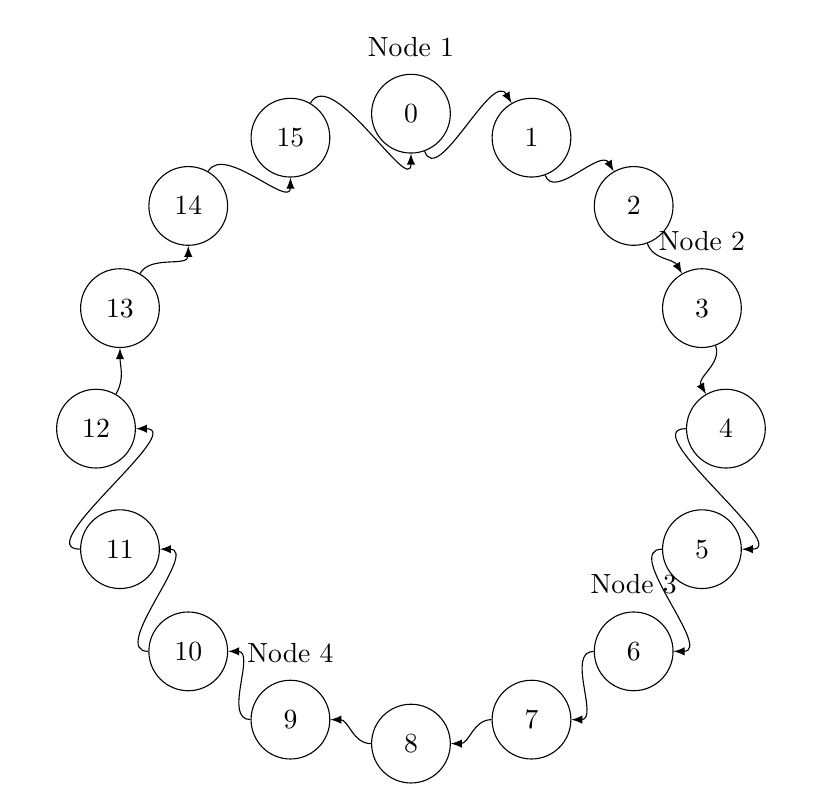
\begin{tikzpicture}
  % Define nodes
  \foreach \i/\k in {0/4,1/3,2/2,3/1,4/0,5/15,6/14,7/13,8/12,9/11,10/10,11/9,12/8,13/7,14/6,15/5}
    \node[circle,draw,minimum size=1cm] (\i) at (\i*360/16:4cm) {\k};

  % Draw connections
  \foreach \i/\j in {8/9,9/10,10/11,11/12,12/13,13/14,14/15,15/0}
    \draw[-latex] (\j) to[out=(180,in=0] (\i);

  \foreach \i/\j in {4/5,5/6,6/7,7/8}
    \draw[-latex] (\j) to[out=60,in=-90] (\i); 

  \foreach \i/\j in {0/1,1/2,2/3,3/4}
    \draw[-latex] (\j) to[out=290,in=120] (\i); 


  % Label nodes
  \node[above=0.1cm of 4] {Node 1};
  \node[above=0.1cm of 1] {Node 2};
  \node[above=0.1cm of 14] {Node 3};
  \node[above=0.1cm of 11] {Node 4};
\end{tikzpicture}
\end{document}
